\documentclass{rapport}
\usepackage{lipsum}
\usepackage{tikz}
\usetikzlibrary{shapes.geometric, arrows}

\title{Rapport Projet Interface} %Titre du fichier

\begin{document}

%----------- Informations du rapport ---------

\logo{logos/Unicaen.png}
\unif{Université de Caen Normandie}
\titre{Jeu de Bataille Navale}


\enseignant{Yan  \textsc{Mathet}\\Christophe \textsc{Charrier}} %Nom de l'enseignants
\jury{Christophe \textsc{Charrier}}

\eleves{Celina \textsc{Bedjou} \\
          Wassim \textsc{Djeha} \\
        Louheb \textsc{Kaced}\\
        Yani \textsc{Belkacemi}} %Nom des étudiants

%----------- Initialisation -------------------
        
\fairemarges %Afficher les marges
\fairepagedegarde %Créer la page de garde
\tabledematieres %Créer la table de matières

%------------ Corps du rapport ----------------
\section{Introduction}


\subsection{Description générale du mini projet}


\large{Le projet vise à développer le jeu de bataille navale qui est un jeu de société classique dans lequel deux joueurs (joueur vs ordinateur) s'affrontent sur une grille de 10x10 cases. Chaque joueur place ses navires sur la grille de manière stratégique, sans que l'adversaire ne puisse les voir, avant de commencer le jeu.







Le jeu de bataille navale est un jeu amusant et stimulant qui exige des compétences de déduction, de stratégie et de tactique pour gagner. C'est un jeu idéal pour deux joueurs, mais il peut également être adapté pour être joué en solo contre une intelligence artificielle.



\section{Objectifs du projet}


Le projet consiste à développer une version du jeu très connu "Bataille Navale" en utilisant les concepts de Java et le modèle MVC (Modèle-Vue-Contrôleur) pour séparer la logique métier, l'interface utilisateur et la gestion des entrées/sorties de manière organisée et structurée.



\subsection{Description des grandes étapes et fonctionnalités à implémenter}


\begin{enumerate}




\item \textsc{Conception du modèle} :


\begin{itemize}


\item Définir les classes pour les bateaux, les cases de jeu, les joueurs, etc.


\item Implémenter la logique du jeu, telle que les règles, la gestion des états des bateaux, les validations, etc.


\item Gérer les interactions avec le contrôleur pour mettre à jour l'état du jeu en conséquence.


\end{itemize}


\item \textsc{Conception de la vue } :


\begin{itemize}


\item Créer les interfaces utilisateur pour afficher les grilles de jeu, les cases, les navires, les indicateurs d'état, etc.


\item Gérer les interactions de l'utilisateur, telles que la sélection d'une case pour tirer un missile, l'affichage des résultats des tirs, etc.


\item Rafraîchir la vue en fonction des mises à jour du modèle.


\end{itemize}


\item \textsc{Conception du contrôleur } :


\begin{itemize}


\item Gérer les événements de l'utilisateur, tels que les clics de souris, les touches du clavier, etc.


\item Valider les entrées de l'utilisateur et communiquer avec le modèle pour mettre à jour l'état du jeu.


\item Rafraîchir la vue pour afficher les changements dans l'état du jeu.



\end{itemize}






\end{enumerate}




\subsection{Organisation et répartition des tâches}


La répartition des tâches pour le projet de développement du jeu de bataille navale, s'est faite de la manière suivante : deux membres travaillent en binôme sur la partie console du jeu, tandis que les deux autres membres travaillent en binôme sur la partie interface utilisateur du jeu ,sauf


L'intégration de la logique de jeu dans l'interface utilisateur en utilisant le modèle MVC pour assurer une séparation claire des responsabilités et faciliter la maintenance et l'évolution du code qui est faite par les 4 membres.

     
   
\section{Comment lancer le jeu}
\subsection{Création du fichier jar}


Tout d'abord on se positionne dans le dossier livraison
\begin{enumerate}
    
    \item il faut créer le fichier \textbf{MANIFEST.MF} ou on met le fichier JAR.
    \item remplacer le contenu du fichier manifest par  \textbf{Main-class: src/demo/Demo } qui sert à determiner la class éxécutable .
    \item Enfin pour créer le fichier JAR on doit taper la commande suivante dans un terminal \textbf{jar cvmf ../../dist/MANIFEST.MF ../../dist/bataille.jar src/cotroller/*.class src/vue/*.class src/demo/*.class src/util/*.class src/model/*.class module-info.class}.

\end{enumerate}
\subsection{Lancement du jeu}
En ce qui concerne le lancement du jeu , il existe deux méthodes pour les 2  On se positionne dans /livraison :
\begin{enumerate}
    \item On compilant tous les fichier avec la commande : \textbf{javac -d build src/model/*.java src/cotroller/*.java src/vue/*.java src/demo/*.java src/util/*.java}
\item  Puis on execute avec la commande  \textbf{java -cp build src.demo.Demo}


\end{enumerate}
ou alors utilisant la 2eme methode :
\begin{enumerate}
    \item Ou alors en éxecutant la commande suivant  : \textbf{"java -jar dist/bataille.jar"} dans un terminal qu'on ouvrira dans le dossier racine livraison.  
\end{enumerate}







\section {Modèle MVC}

\subsection{Architecture du projet}

Dans notre projet, nous avons adopté une structure de données Modèle-Vue-Contrôleur, où le modèle est essentiellement indépendant des autres parties du projet. Lorsqu'une entrée clavier ou souris est détectée, le modèle demande à la vue de solliciter le contrôleur, car la méthode d'accès aux entrées varie en fonction de la vue utilisée
\begin{figure}[h]
\centering
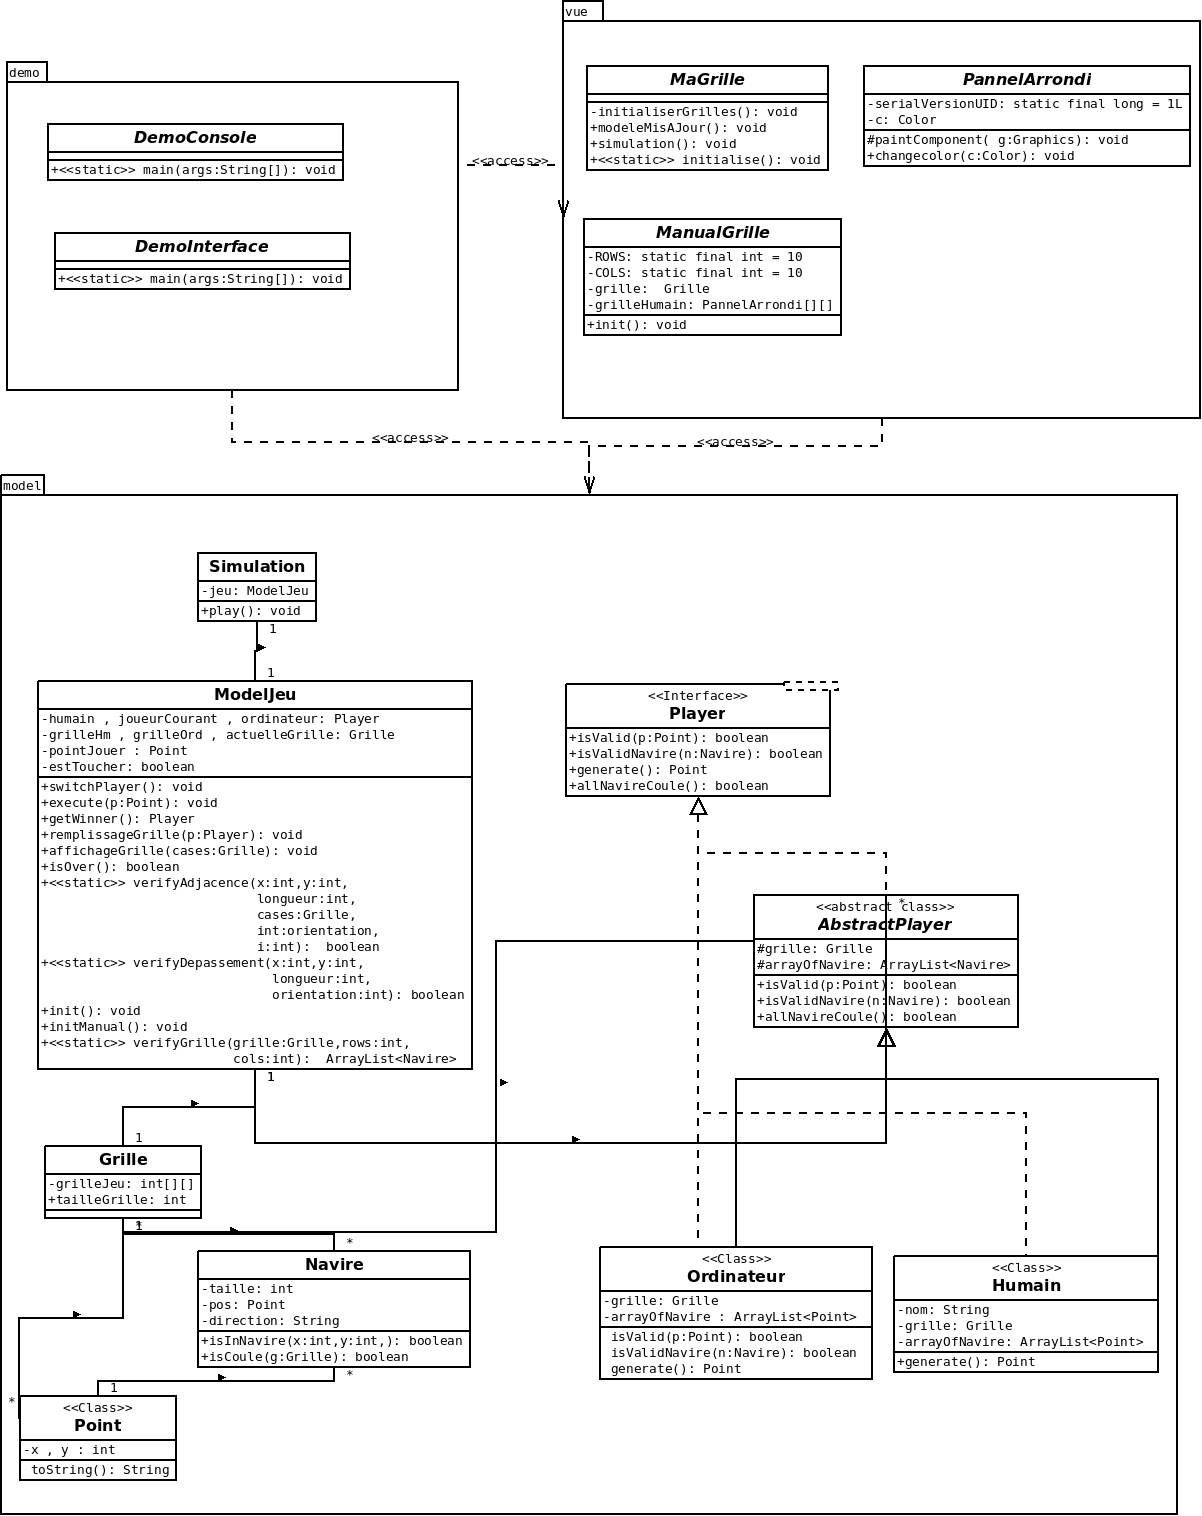
\includegraphics[scale=0.3]{images/InterfaceGraphique.png}
\caption{Architecture du projet}
\end{figure}
\newpage

Les flèches dans le diagramme  sont utilisées pour représenter les différentes relations entre les classes, les interfaces et les autres éléments dans un diagramme de classes:
\begin{itemize}
    \item[*] Héritage : Une flèche solide dirigée de la classe fille (Comme Classe humain) vers la classe (AbstactPlayer).
    \item[*] Interface : Une flèche pointillée dirigée de la classe implémentant l'interface(AbstactPlayer) vers l'interface(Player)
\end{itemize}

\begin{figure}[h]
\centering
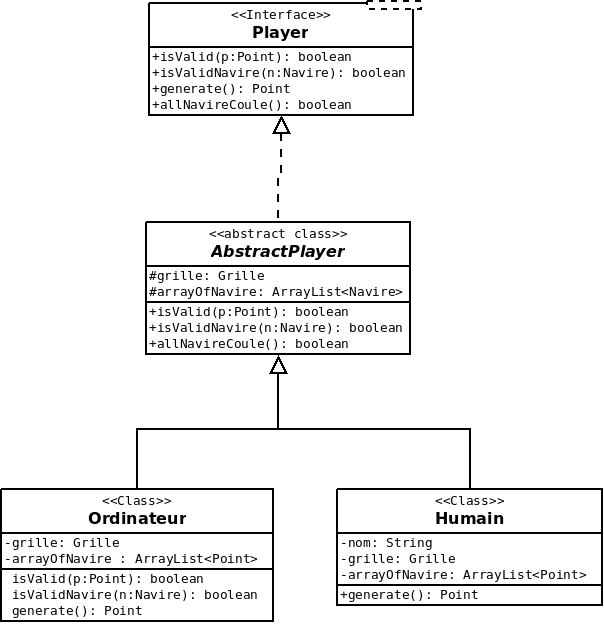
\includegraphics[scale=0.3]{images/api.png}
\caption{Exemple d'utilisation Interface/Heritage dans notre projet }
\end{figure}
\subsection{L'Organisation en MVC de notre projet}
La vue et le modèle des joueurs de notre projet sont organisés de cette manière :\\
\begin{figure}[h]
\centering
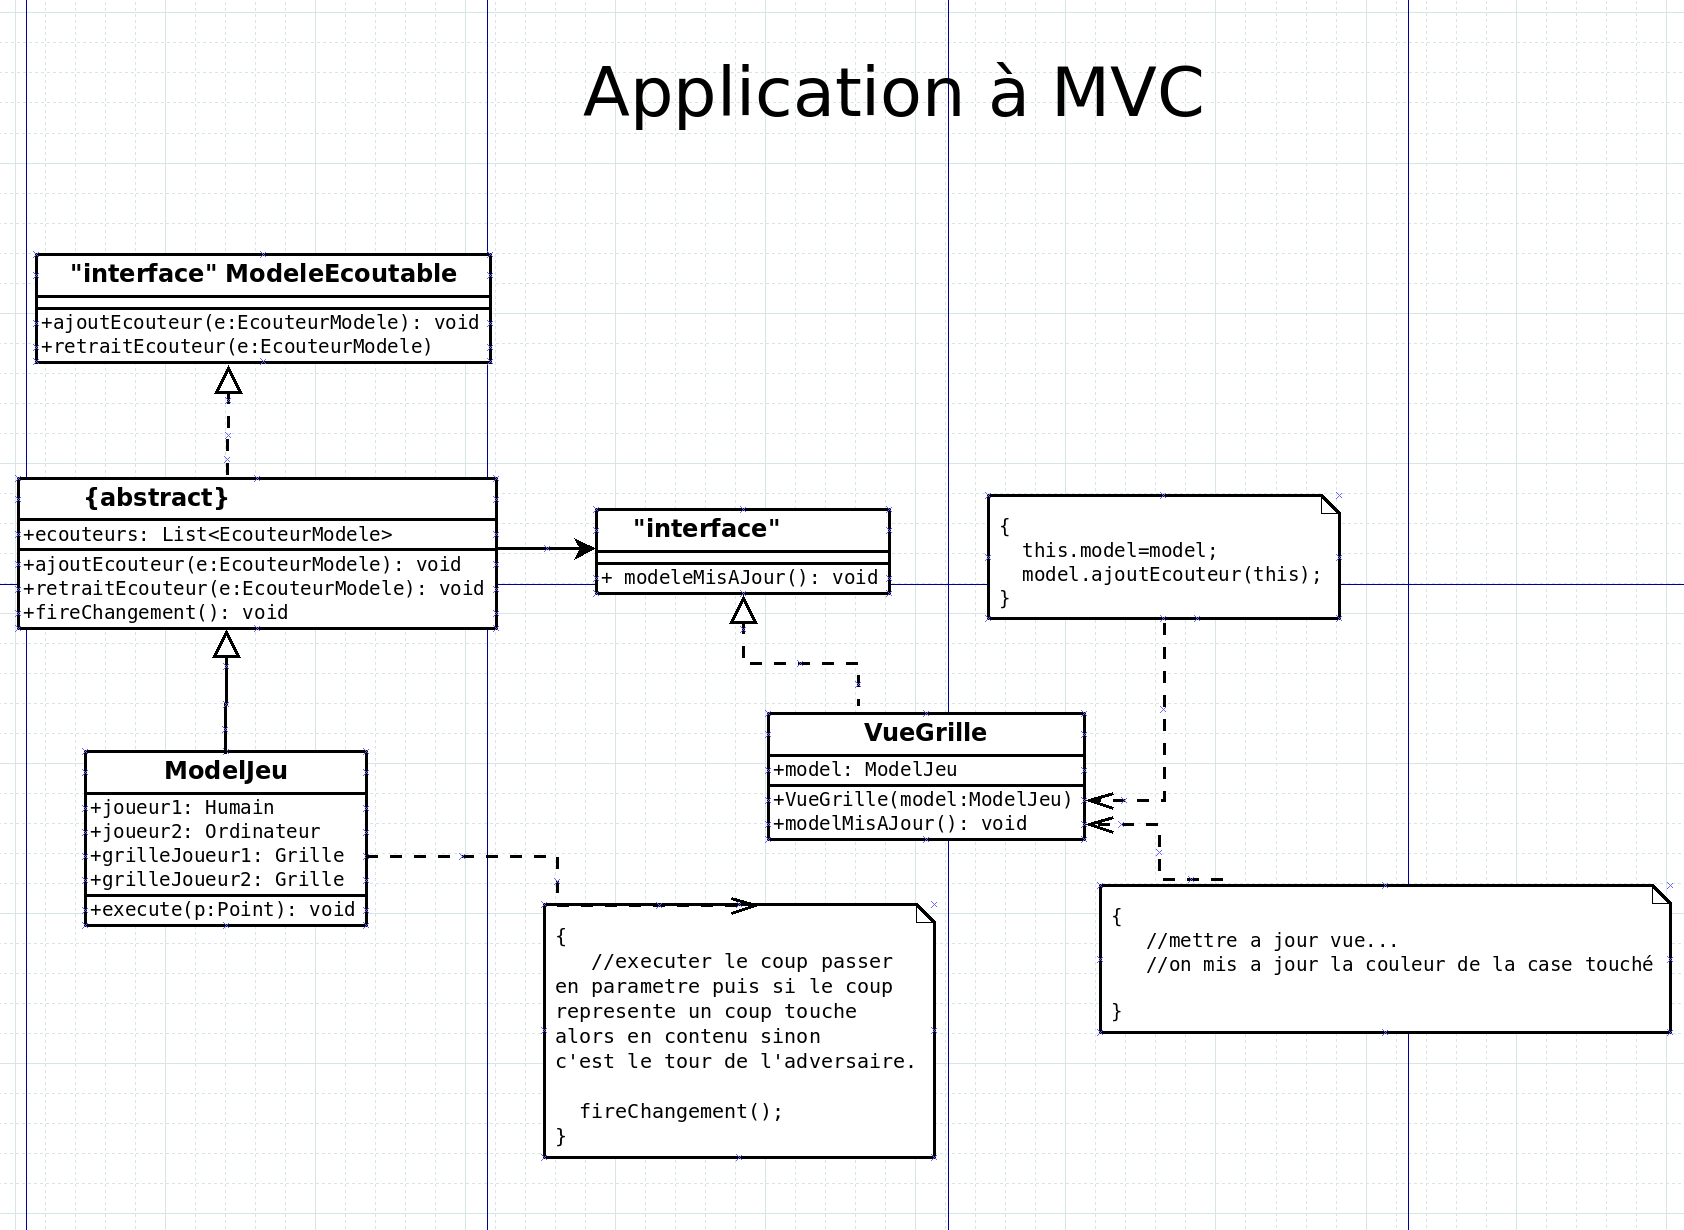
\includegraphics[scale=0.3]{images/MVC.png}
\caption{Organisation MVC}
\end{figure}
Selon l'approche du modèle MVC que nous avons suivie, nous avons souhaité créer un code qui tire parti des fonctionnalités offertes par Java afin d'éviter d'avoir du code "en dur" ou codé en dur. Nous avons cherché à rendre notre code modulable, de manière à permettre l'implémentation d'un algorithme de résolution par une personne externe au projet. Pour ce faire, il lui suffit d'implémenter une nouvelle classe qui héritera de la classe "ModeleJeu" ou bien d'ajouter directement l'algorithme en questions dans la classe "ModeleJeu" et d'y ajouter ses propres algorithmes.

De même, si cette personne souhaite retravailler les vues de l'application, elle peut implémenter une nouvelle classe qui hérite de "EcouteurModele",puis de redéfinir la méthode miseAjour en l'adaptons à la conception du jeu.
\section{Interactions avec les différentes vues }
Dans notre projet, nous avons implémenté deux types d'interactions avec les différentes vues : le Console et l'Interface.





\subsection{Console}
\textbf{Console} : l'utilisation du mode "Terminal" permet ,d'une part aux utilisateurs (non-IA) de jouer directement via la console , puis le programme demande au joueur de placer ses navires en choisissant les coordonnées (en entrant un chiffre entre 0 et 9 pour chaque axe) et leur direction. Si un joueur tente de placer un navire qui dépasse du plateau de jeu ou qui se superpose avec un autre navire, le programme demande de recommencer le placement ,d'autre part il permet à l'ordinateur utilisateur (IA) de remplir ça grille de navires aléatoirement avec la méthode "remplissageGrille()" qui gère les collisions des bateaux .

Ensuite ,une fois que l'ordinateur a fini de placer ses navires, son plateau est masqué . Une fois que tous les navires sont placés, vient le moment de choisir les coordonnées pour les tirs. L'humain entre les coordonnées au clavier de 0 à 9 pour les axes X (abscisses) et Y (ordonnées) est l'ordinateur le fait aléatoirement, .

Le terminal utilise une syntaxe spécifique pour afficher l'état du jeu :
\begin{enumerate}
    \item "!" pas de navire
    \item "1" indique les navires du joueur
    \item "\_" indique de l'eau ou un navire masqué
\end{enumerate}



Le programme se termine dès qu'un joueur remporte la partie en affichant le gagnant le nom du joueur.

\begin{figure}[h]
\centering
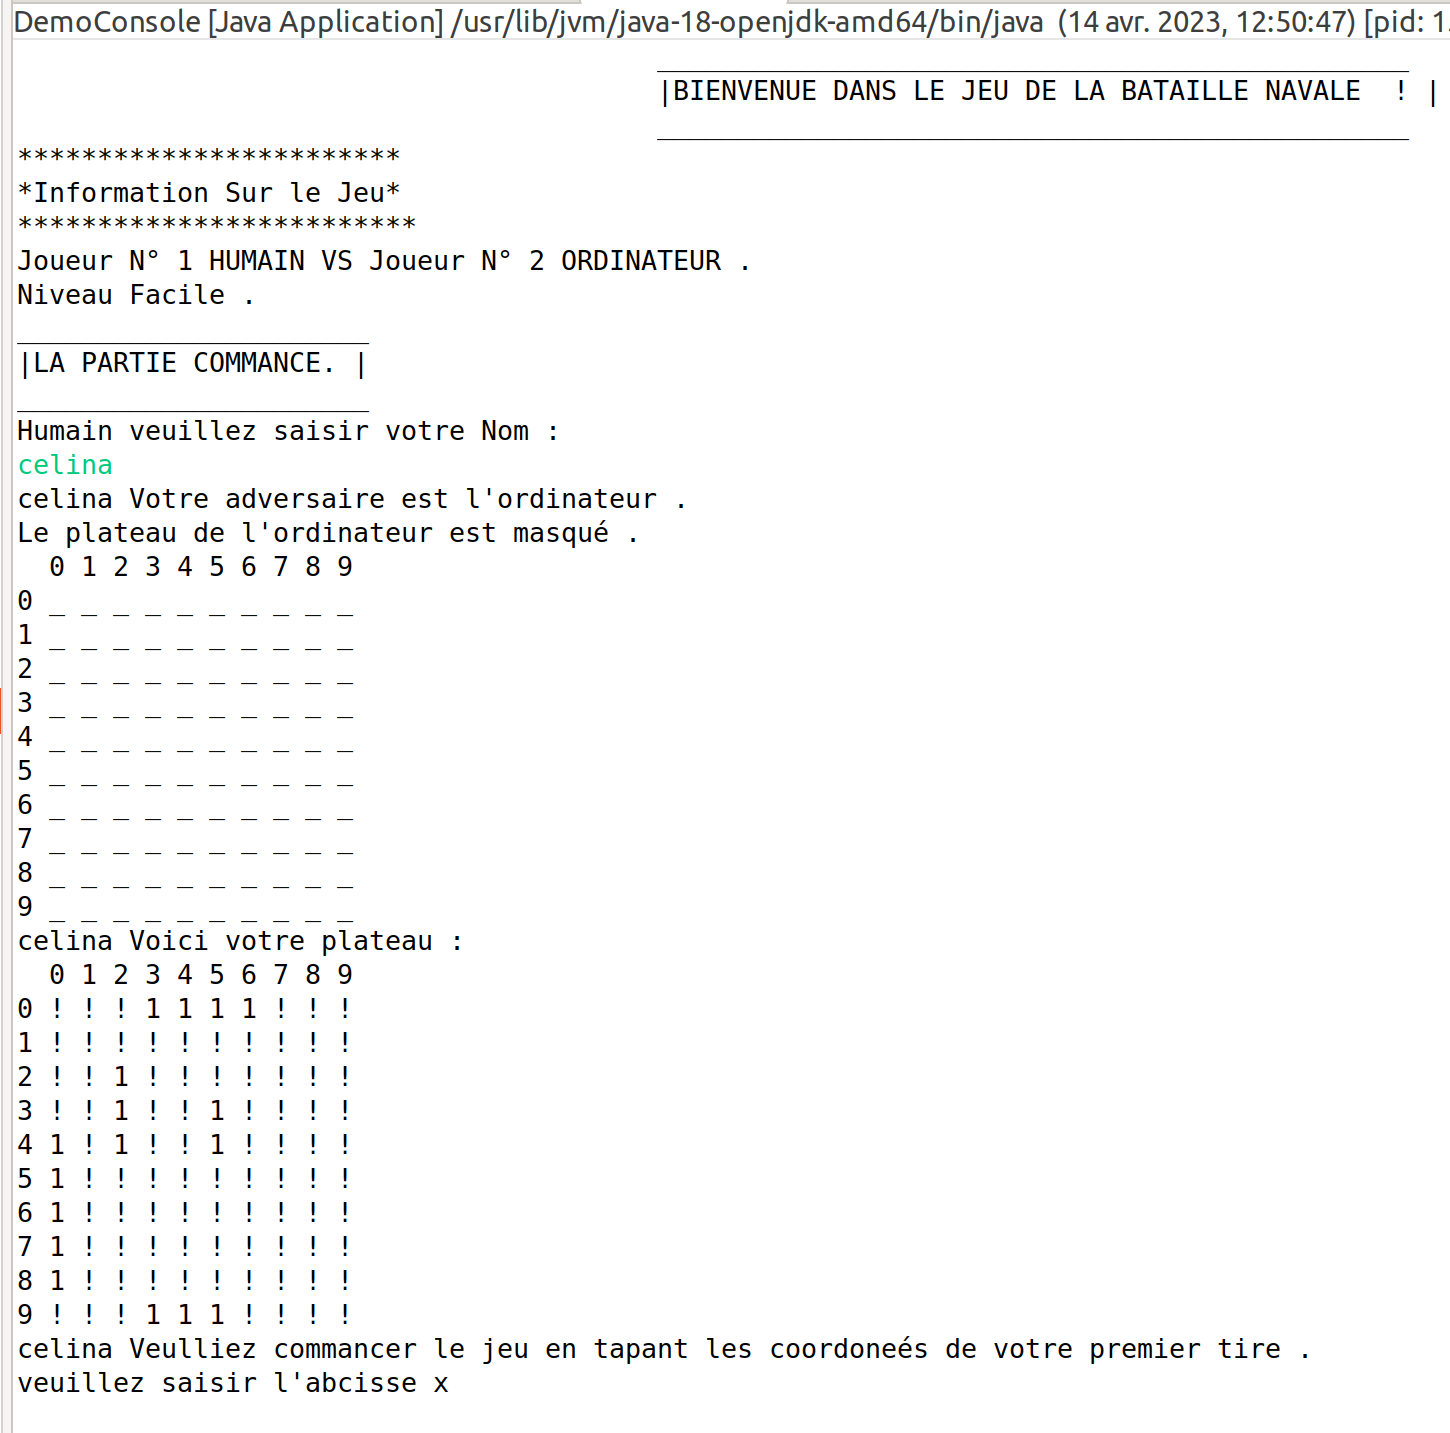
\includegraphics[scale=0.3]{images/DemoConsole.png}
\caption{Affichage Console de notre jeu }
\end{figure}
\newpage
\subsection{Interface}
\textbf{Interface} : le mode "Interface" permet aux utilisateurs (IA et non-IA) de jouer à travers une interface composée de deux grilles, une pour chaque joueur. Le programme demande au joueur Humain de placer ses navires en choisissant les coordonnées en cliquant directement sur une des cases de la grille en suivant les règles du jeu. Si les joueurs tentent de placer un navire qui ne rentre pas entièrement dans sa grille ou qui se superpose avec un autre navire, le programme demandera de recommencer le placement.

Ensuite, une fois que le joueur Humain a fini de placer ses navires, l'ordinateur place ses navires de façon aléatoire en appelons la fonctions "rempissagegrille()" . Une fois que tous les navires sont placés, la grille du joueur adverse est masquée et vient le moment de choisir les coups.


Le joueur sélectionne les cases de la grille en cliquant dessus c'est-à-dire en cliquant sur le plateau blue.

Les navires sont représentés par une couleur rouge pour indiquer leur direction :
\begin{itemize}
\item Un rond rouge = navire TOUCHE.
\item Un rond vert = coup raté (pas de navire)
\item le blue indique de l'eau .
\end{itemize}



Un navire coulé reste affiché à l'écran. Le programme se termine dès qu'un joueur remporte la partie.
\begin{figure}[h]
\centering
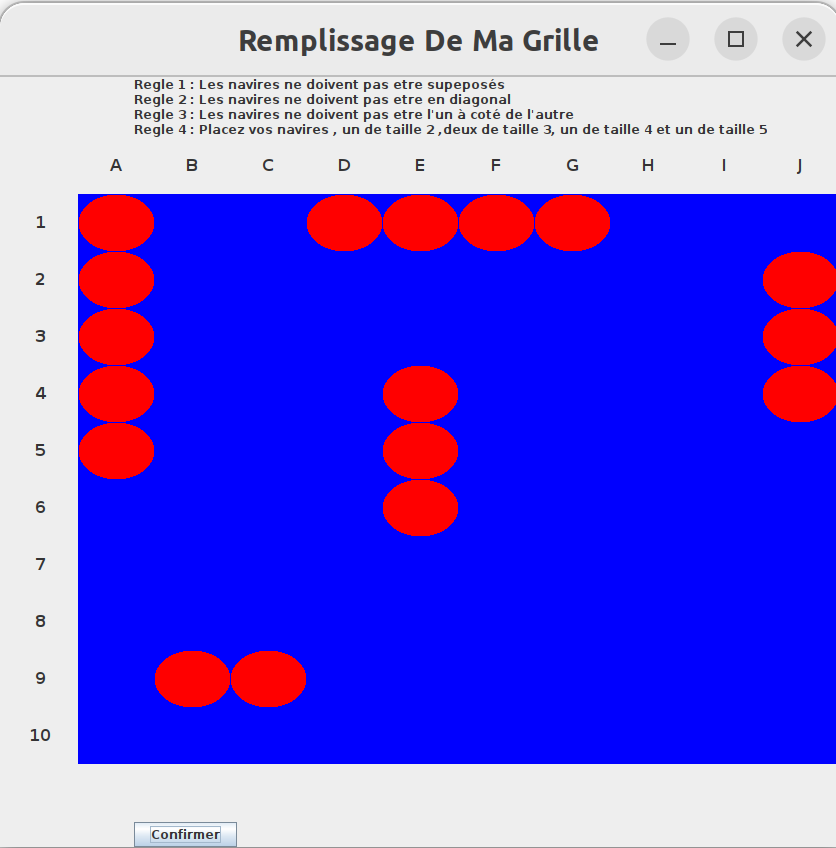
\includegraphics[scale=0.3]{images/remplissage.png}
\caption{Exemple remplissage de la grille humain avant le debut de la partie }
\end{figure}
\begin{figure}[h]
\centering
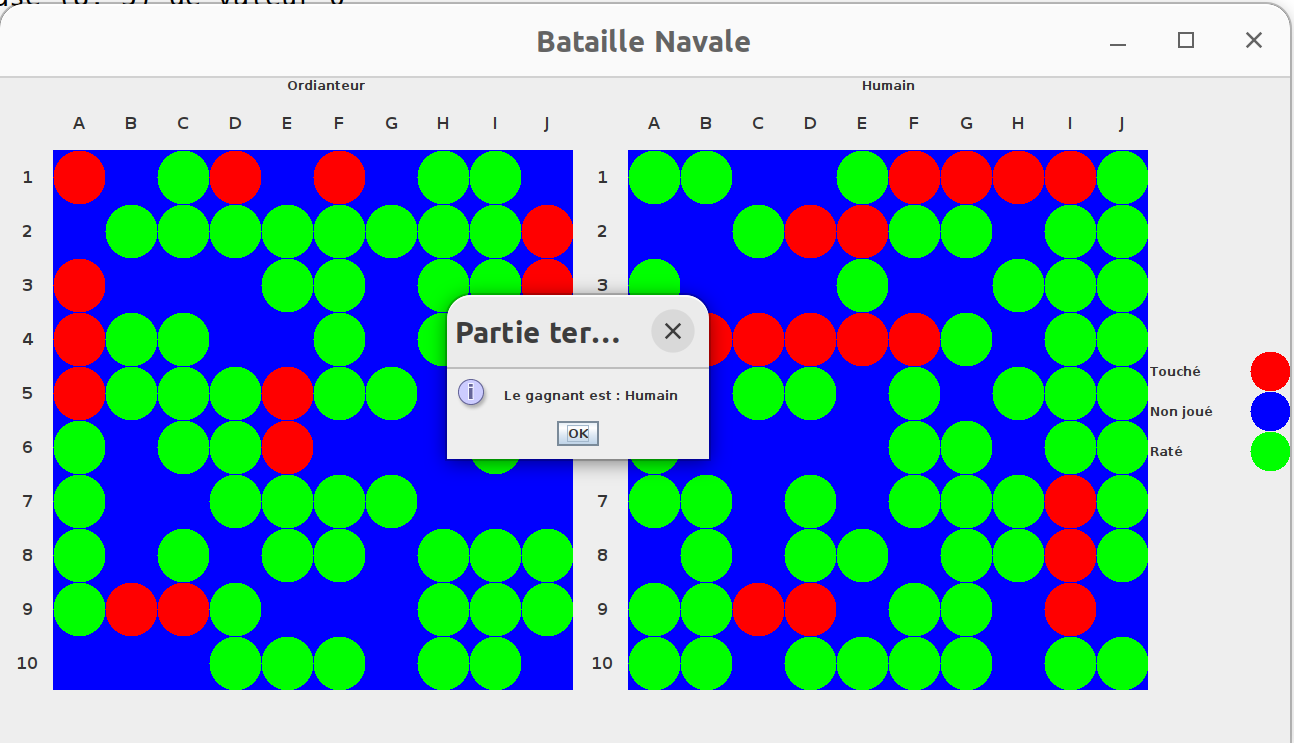
\includegraphics[scale=0.3]{images/DemoInterface.png}
\caption{Exemple fin d'une partie bataille navale ,gagnant l'humain}
\end{figure}
    \subsection{Améliorations faites}
            \begin{enumerate}
                \item L'implémentation de fonctionnalités avancées dans le jeu de bataille navale peut inclure la possibilité de jouer contre l'ordinateur avec une intelligence artificielle basique. Par exemple, lorsque l'ordinateur choisit un coup aléatoire sur la grille de l'adversaire, il vérifie d'abord si la case choisie a déjà été sélectionnée en consultant la grille pour voir si elle contient un 2. Si c'est le cas, l'ordinateur choisit un autre coup aléatoire. Si la case contient un 1, alors cela signifie qu'un bateau a été touché, et si la case contient un 0, cela signifie que le coup a été raté. En fonction de ces informations, l'ordinateur ajuste sa stratégie et prend une décision éclairée pour son prochain coup. La mise en œuvre de cette fonctionnalité peut nécessiter la manipulation de données de grille, la génération de nombres aléatoires et la logique de prise de décision pour l'ordinateur afin de simuler une intelligence artificielle basique dans le jeu.\\
                Voici La fonction "execute(Point p)"  est une méthode pour gérer la logique de jeu de la bataille navale entre un joueur humain et un joueur ordinateur. \\Voici une description générale de ce que cette fonction fait :
\begin{enumerate}
    \item Vérifier si c'est le tour du joueur humain ou de l'ordinateur en comparant le joueur courant avec le joueur humain.
    \item Si c'est le tour du joueur humain :
        Vérifier si la case choisie par le joueur humain (représentée par l'objet "Point p") contient un navire de l'ordinateur en vérifiant la valeur de la case dans la grille de l'ordinateur. Si c'est le cas, marquer la case comme touchée (en modifiant la valeur de la case dans la grille de l'ordinateur à 2) et définir la variable "esttoucher" à vrai.
        Afficher un message indiquant que le coup du joueur humain est un coup "TOUCHE".
        Sinon, définir la variable "esttoucher" à faux, afficher un message indiquant que le coup du joueur humain est un coup "RATE", et passer au tour du joueur suivant en appelant la fonction "switchPlayer()" pour changer le joueur courant.
        \item Sinon, si c'est le tour de l'ordinateur :
        Vérifier si la case choisie par l'ordinateur (représentée par l'objet "Point p") contient un navire du joueur humain en vérifiant la valeur de la case dans la grille du joueur humain. Si c'est le cas, marquer la case comme touchée (en modifiant la valeur de la case dans la grille du joueur humain à 2) et définir la variable "esttoucher" à vrai.
        Afficher un message indiquant que le coup de l'ordinateur est un coup "TOUCHE".
        Sinon, si la case choisie par l'ordinateur ne contient pas de navire du joueur humain (représentée par la valeur 1 dans la grille du joueur humain), marquer la case comme jouée (en modifiant la valeur de la case dans la grille du joueur humain à 2) pour éviter que l'ordinateur ne choisisse la même case à nouveau, définir la variable "esttoucher" à faux, afficher un message indiquant que le coup de l'ordinateur est un coup "RATE", et passer au tour du joueur suivant en appelant la fonction "switchPlayer()" pour changer le joueur courant.
        \item Mettre à jour la variable "pointjouer" avec la valeur de "Point p".
    Appeler la fonction "fireChange()" pour notifier les éventuels écouteurs ou observateurs d'un changement dans l'état du jeu.
\end{enumerate}
    
    
    
\end{enumerate}
           
    \subsection{Améliorations possibles}
            Les améliorations possibles pour le projet de bataille navale comprennent :
\begin{enumerate}
    \item  Amélioration de l'IA de l'ordinateur pour offrir un défi plus difficile aux joueurs en utilisant des algorithmes de recherche avancés.
    \item Ajout de fonctionnalités multijoueurs pour permettre aux joueurs de jouer en mode multijoueur, en local ou en ligne.
   
    
\end{enumerate}

   
\section{Conclusion}
    En conclusion, le développement du jeu de bataille navale en utilisant les concepts de Java et le modèle MVC a été un projet passionnant et stimulant. Ce projet a permis aux membres de l'équipe de renforcer leur compréhension des concepts de programmation en Java, ainsi que de se familiariser avec le modèle MVC pour organiser et structurer le code. La collaboration étroite entre les membres de l'équipe a été essentielle pour atteindre les objectifs du projet et garantir une cohérence dans l'expérience utilisateur du jeu.\\
    En conclusion, le jeu de bataille navale développé en utilisant Java et le modèle MVC constitue un exemple réussi d'application pratique des concepts de programmation et de conception de logiciels. Il offre une expérience de jeu intéressante pour les joueurs, tout en démontrant la maîtrise des compétences techniques et la capacité à collaborer en équipe dans un projet de développement logiciel.
    


       
       
\end{document}